\section{目的}
依PDF91--93頁完成Lab23，除了2-to-4負載比較，補做3-to-8與兩種8-to-256架構；不只模擬少數代表輸出。

\section{Spec 對照}
S 表示已執行模擬檢查，D 表示分析與討論。

\small\begin{longtable}{p{.46\linewidth}p{.30\linewidth}p{.15\linewidth}}\toprule
要求與 PDF 頁碼 & 對應 deck／檢查 & 狀態 \\ \midrule\endhead
NAND/NOR 2-to-4，10fF（91--93） & D01/C0 & S \\
增加負載與級數問題（93） & D01/C1--3 & S+D \\
設計3-to-8（93） & D02; 8 codes & S \\
兩級與三級8-to-256（93） & D03; 256 codes each & S \\
階層架構delay/power比較（93） & D04; 10/100fF & S+D \\
\bottomrule\end{longtable}\normalsize


\section{電路與設計推導}
2-to-4的NAND型為四個NAND2加四個輸出inverter；NOR型為四個NOR2，兩者均含兩個輸入反相器。共28與20顆MOS，負載每輸出10 fF。3-to-8用八個NAND3+inverter及三個輸入反相器，共70顆MOS。

兩級8-to-256先把低／高4-bit各解成16個predecode，再以256個AND2組合。三級先用四個2-to-4，再組成兩個4-to-16，最後AND2輸出。此處「級」指邏輯分解；每個正AND實作為NAND+inverter，所以不含輸入反相器的電氣gate level分別為4與6；補數輸入路徑多經一個inverter，合計5與7級。含輸入反相的MOS數為1872、1840。中間4-to-16組合gate採2倍尺寸以驅動16個末級負載；其餘單位 $W_p/W_n/L=3.6/1.8/0.25\,\mu$m，串聯NMOS或PMOS按stack等比加寬。

\section{模擬設定}
模型由使用者於本機另行提供；採 1 V、27 $^\circ$C 的教學適配條件，不把講義舊製程的 2.5 V 數值視為本次通過門檻。使用 PrimeSim HSPICE S-2021.09、\texttt{accurate}、\texttt{runlvl=5}，由實際 \texttt{.print/.measure} 數據繪圖。每個 \texttt{.alter} 重設全部基準參數與溫度。所有案例皆完成，無 error 或 failed 量測；這不代表完全沒有模型或收斂提示。公開 netlist 僅保留 \texttt{* MODEL\_SETUP\_REQUIRED} 註解，不附模型路徑。完整數據位於該 lab 的 \texttt{results/}，大型資料依 deck 分檔，由 \texttt{simulation\_data.json} 索引。四份deck共八案例。2-to-4枚舉0/1/2/3並重複，每碼2 ns、20 ps邊緣；負載10/50/100/500 fF、最大1 ps步距。每碼80\%處檢查一熱輸出，logic0/1門檻0.1/0.9 V。3-to-8與兩種8-to-256用DATA DC sweep列出所有輸入碼及所有輸出。8-to-256 transient採0,1,0,15,255,0,16,0，每碼5 ns、最大2 ps步距，delay明確取0到1及1到0的output1。

\section{結果與規格檢查}
\begin{center}\small\begin{tabular}{lrrrr}\toprule
Load (fF) & NAND rise/fall (ps) & NOR rise/fall (ps) & NAND/NOR P ($\mu$W) & Fails \\ \midrule
10 & 112.4/156.1 & 155.0/62.6 & 54.8/55.6 & 0 \\
50 & 213.9/201.9 & 254.0/107.6 & 76.2/77.8 & 0 \\
100 & 331.7/248.1 & 371.4/156.7 & 101.9/103.6 & 0 \\
500 & 1259.8/396.7 & 1289.6/236.6 & 237.5/233.7 & 16 \\
\bottomrule\end{tabular}\end{center}

\begin{figure}[htbp]\centering
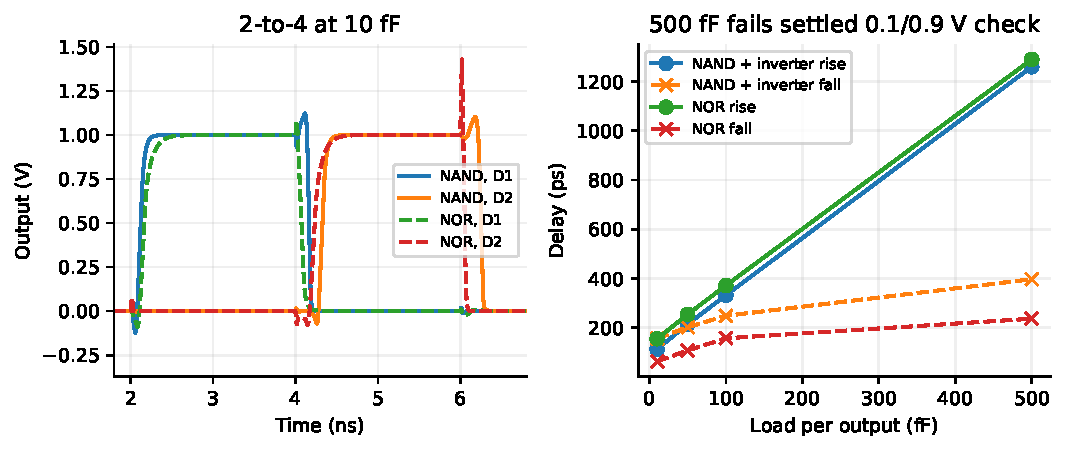
\includegraphics[width=\linewidth]{figures/decoder_load.pdf}
\caption{2-to-4波形與負載關係；500 fF於指定2 ns碼寬下未達穩態rail門檻。}
\end{figure}
\begin{center}\small\begin{tabular}{lrrrr}\toprule
Load (fF) & Stages & $t_{rise}$ (ps) & $t_{fall}$ (ps) & $P$ ($\mu$W) \\ \midrule
10 & 2 & 744.7 & 590.3 & 522.7 \\
10 & 3 & 1360.2 & 924.9 & 238.8 \\
100 & 2 & 964.9 & 693.7 & 552.7 \\
100 & 3 & 1579.8 & 1028.3 & 257.1 \\
\bottomrule\end{tabular}\end{center}

\begin{figure}[htbp]\centering
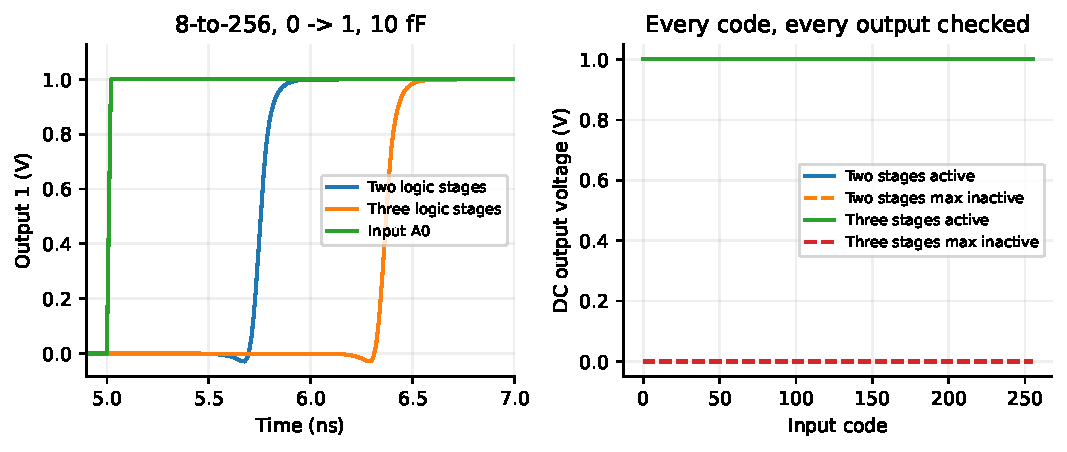
\includegraphics[width=\linewidth]{figures/hierarchical_decoder.pdf}
\caption{8-to-256的代表性轉態與每一碼、每一輸出的DC真值驗證。}
\end{figure}
3-to-8全部8碼通過；兩種8-to-256各256碼、全部輸出均符合一熱真值表，共512組架構／輸入檢查。DC大型網路有收斂重試提示，但最終完成且所有真值檢查通過，未刪除失敗碼後報成功。

2-to-4在10/50/100 fF的每個穩態檢查皆通過；500 fF在18個架構／時槽檢查中有16個未達0.1/0.9 V，因此該碼率下不能宣稱有效數位輸出。其50\% delay仍能量到，與完整邏輯rail成功是不同判準。

\section{討論}
固定負載時，增加級數不一定增加delay：額外buffer可分配fanout、改善transition，但也增加intrinsic delay與切換電容。此處8-to-256兩級的10 fF上升delay約744.7 ps，三級約1360.2 ps；三級在本stimulus的供應功率較低（238.8 vs 522.7 $\mu$W），不構成通用速度／功率定理。尺寸、stack阻抗、輸入電容、fanout及活動率都會改變排序。

NAND型2-to-4雖多一級，這裡上升較快；NOR型下降較快，不能只用單一edge概括整體delay。多位同時改變會有hazard，真值表只驗證穩定後的選擇；時序圖保留尖峰。階層decoder未加入佈線、抽取寄生或實體版圖，所以晶體管數只用作拓樸成本。

\section{結論}
講義三種規模的decoder皆完成，包含完整256-code真值檢查。重負載失效與動態hazard如實保留；兩級／三級比較只適用於已明列的邏輯分解、尺寸、負載與活動。
